\section{Experimental Evaluation}\label{sec:evaluation}
In Section \ref{sec:practical-results-lit}, we looked at other results in the literature that gave a decent comparison between some of the algorithms; however, we did not learn much about the datasets, especially the structure of the preference list and distribution of those preferences. Therefore, we are conducting experiments by benchmarking the implemented algorithms with both real and artificial datasets of varying sizes and preference structures.

\subsection{Research Questions}\label{sec:research-q}
Table \ref{tab:algorithm-comparison} already compared and summarized the algorithms from a theoretical perspective; however, some of the results would benefit from further quantification and clarity. For instance, we know that the Popular-CHA algorithm, as described in Section \ref{algo-max-pop}, does not always produce a matching. It would be beneficial to empirically investigate if certain inputs cause this problem. Therefore, we formalize some open questions as research questions that these experiments try to answer:
\begin{enumerate}
    \item What is the effect of different preference distributions on the matchings produced by the different algorithms?
    \item How likely is it for Popular-CHA to not produce a matching using different datasets?
    \item How does the Modified-Popular-CHA algorithm from Section \ref{impl:mod-max-pop} compare in terms of popularity to the other algorithms?
    \item What is the cost of giving up on strategy proofness in terms of rank, i.e. how well does RSD perform compared to other mechanisms?
    \item Is popularity a meaningful metric for the student-seminar use case?
    \item What is the impact of short-preference lists on the quality and existence of matchings?
\end{enumerate}

\subsection{Experimental Setup}
The goal of these experiments is quantifying some of the optimality criteria defined in Section \ref{sec:optimality} to compare the selection of algorithms empirically and find answers to the research questions proposed in the previous subsection. Due to the fact that real-world data for student enrollments is not widely available, it is important to note that the results of this experiment are biased by the selection of data available - however, by using the available real datasets and a few different synthetic datasets, it should be possible to find answers to the proposed research questions and to better understand the differences of different approaches.

\subsubsection{Benchmark Setup}
The experiments are performed by a Kotlin program that generates test data and then executes each of the algorithms with the same input. The program then collects the results and computes statistics, which are saved into a file. When using synthetic data, the program generates between 10-50 different instances to account for the randomness, but only one instance runs at a time to allow for ideal CPU utilization. All experiments are run on a workstation with an Intel Core i5 8250U processor and 16GB of memory. The following types of instances are being used:
\begin{enumerate}
  \item Real-world datasets
  \item Small, synthetic datasets ($\sim$200 students) with real-world similar preferences
  \item Large, synthetic datasets ($\sim$2500 students) with real-world similar preferences
  \item Large, synthetic dataset with uniform and incomplete preferences (5000 Students)
  \item Large, synthetic dataset with uniform and complete preferences (5000 Students)
\end{enumerate}

\subsubsection{Sample Data}
Due to the fact that real data for seminar registrations is mostly kept private, a majority of the benchmark will rely on synthetic data. However, there are a few publicly available datasets available that will be used for evaluation and also for better understanding real-world preference distributions.

\paragraph{Using Graph Generators}
Using graph generators to synthetically create instances to the seminar-student matching problem turns out to be a big challenge. Essentially, we need a graph generator for bipartite, weighted graphs, that also considers seminar capacities. One option is generating as many nodes as the total capacity of all seminars plus students, but that could result in having duplicate edges, i.e. preferences in the generated instance. Therefore, we instead use a custom, domain specific mechanism for generating instances.

\paragraph{Random Uniform Preference Lists}
Probably the simplest way to synthetically generate data is picking a size for the instance and then generating seminars and students based on a uniform random generator. The preference lists are created by shuffling the list of all seminars for each student. Additionally, we can simply shorten each preference list by a random factor as well to measure the effect of incomplete-preference lists.

\paragraph{PrefLib Datasets}
Preflib.org is an open collection of more than 3000 community-contributed datasets of preference data for different domains \cite{PrefLib}. Fortunately, there exist two datasets of students' course preferences at the Polish AGU University \cite{preflib-dataset}. The two datasets contain strict and complete preference orders for each dataset with 9 courses and 146 students, or 7 courses and 153 students respectively. Unfortunately, there are no capacities given; however, those can easily be computed synthetically. An interesting characteristic of those datasets is that in each dataset, all students rank the same seminar with their first preference. We remove these seminars from the dataset, as to not assume such a preference distribution in the real world.

\begin{figure}[h!]
  \centering
  \begin{subfigure}[b]{0.45\linewidth}
    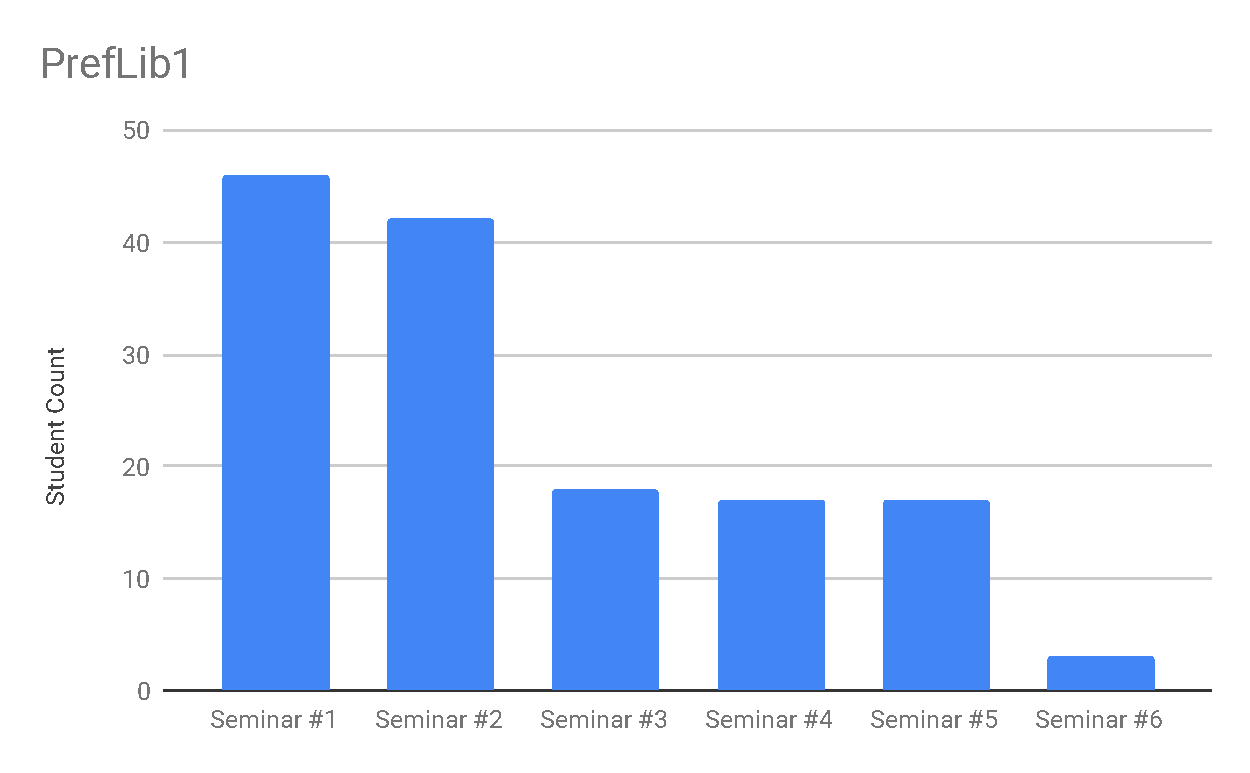
\includegraphics[width=\linewidth]{assets/plots/preflib1-distr.pdf}
    \caption{PrefLib1 Dataset}
  \end{subfigure}
  \begin{subfigure}[b]{0.45\linewidth}
    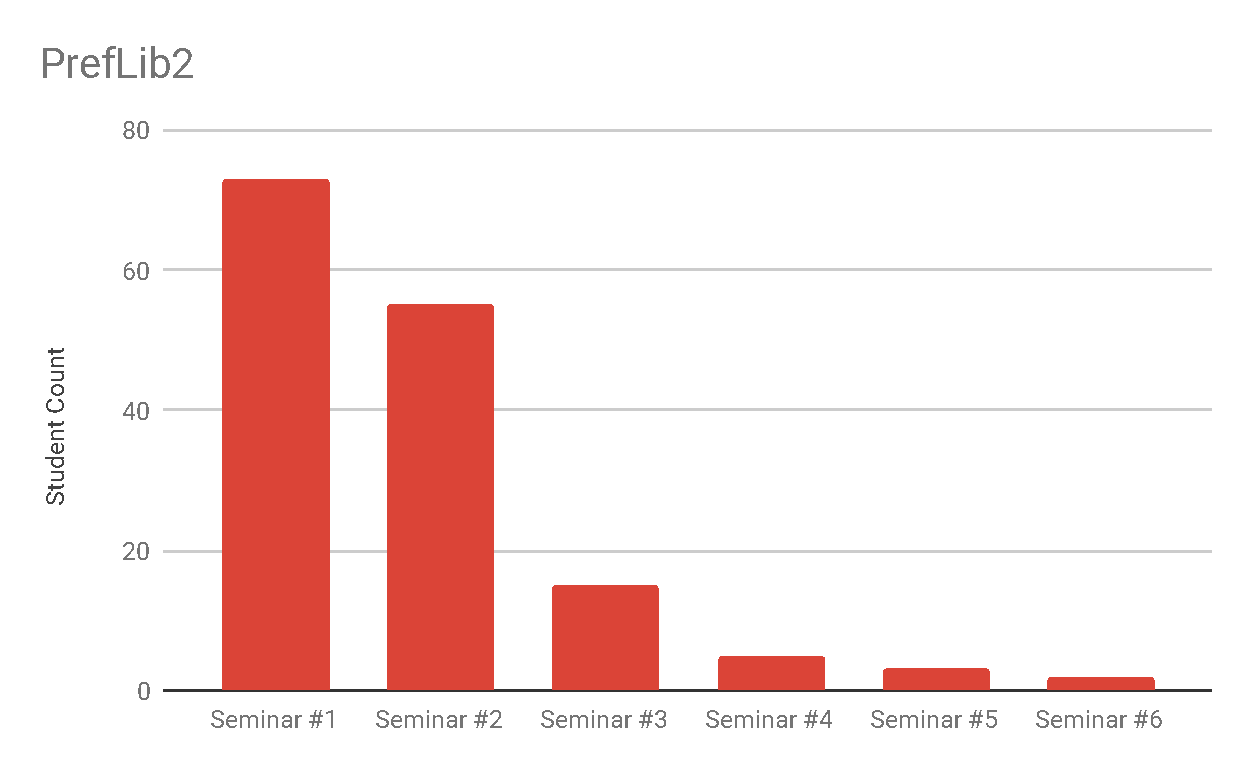
\includegraphics[width=\linewidth]{assets/plots/preflib2-distr.pdf}
    \caption{PrefLib2 Dataset}
  \end{subfigure}
  \caption{Preference Distributions for First-Ranked Seminars for Both PrefLib Datasets}
  \label{fig:preflib-distribution}
\end{figure}

Figure \ref{fig:preflib-distribution} shows the preference distribution for the student's first choice seminars in both datasets after removing the always first-ranked seminar. We can see that in both datasets, students clearly strongly prefer two seminars. In the first dataset, however, there are three more seminars that are also decently popular, while in the second dataset the majority of students really prefers the two dominant seminars. Generally, those datasets indicate that the preference structure of real-world datasets is not likely to be uniformly distributed.

\paragraph{Random Zipf-Distributed Preference Lists}
To better simulate real-world preference structures than by using a uniform distribution, a power law distribution can be applied. One type of power law distributions are \emph{Zipfian Distributions} \cite{Zipf}, which can be used for creating synthetic seminar distributions. Using this type of distribution with some additional randomization yields the following (Figure \ref{fig:zipfian-distribution}) preference list structure when seminar and student counts are similar to the first PrefLib dataset.

  \begin{figure}[h!]
    \centering
    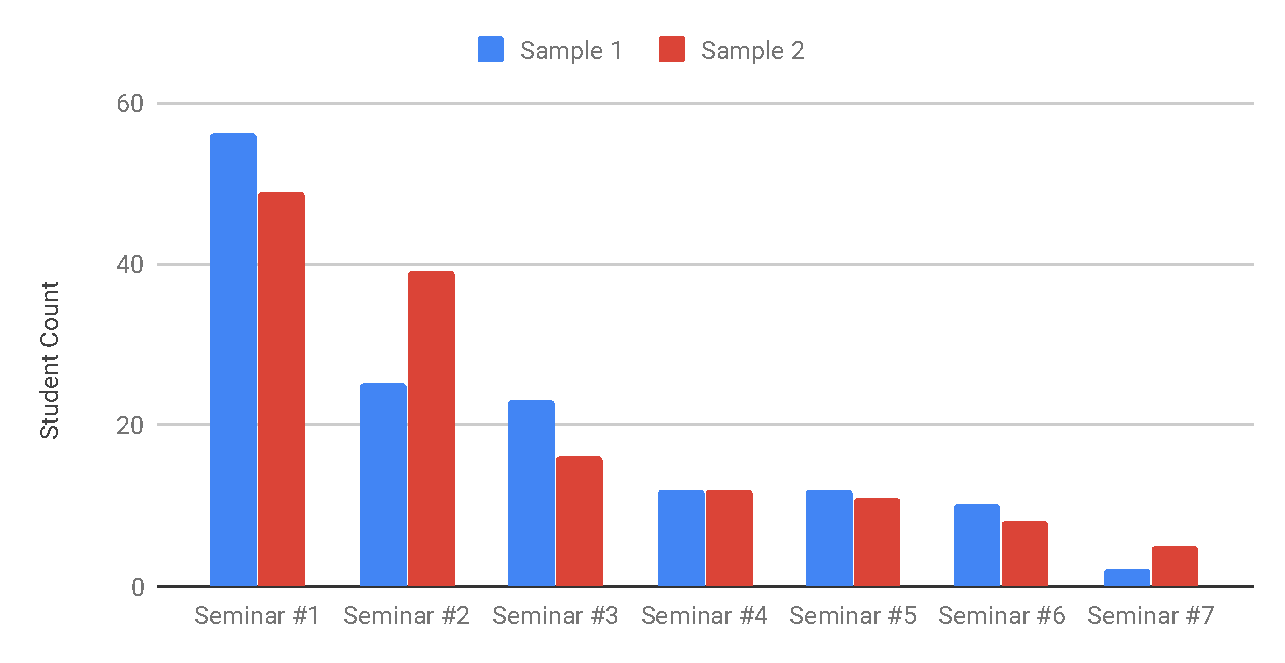
\includegraphics[width=0.6\linewidth]{assets/plots/zipfian-distr.pdf}
    \caption{Two Sample Zipfian Preference Distributions for First-Ranked Seminars}
    \label{fig:zipfian-distribution}
\end{figure}

To create the dataset for each student, a seminar is randomly drawn using the Zipfian distribution and added to his preference list until the desired preference-list length has been reached. Comparing Figure \ref{fig:zipfian-distribution} to Figure \ref{fig:preflib-distribution} shows somewhat similar results, which should make this generator relevant for the benchmark. 

\subsubsection{Metrics}
We already know that all of the algorithms under consideration produce pareto-optimal matchings; however, it will also be necessary to measure popularity. If the Popular-CHA algorithm finds a matching, we know that it is the popular matching, but if the algorithm cannot find a matching, it could be possible that one of the other algorithms produces such a matching. In general, given the definitions for Popularity that we have used before, it is not possible to check if a given matching is popular without comparing it to all other possible matchings. However, this is infeasible due to the exponential runtime complexity of that comparison, which is why we will just compare the matchings produced by the five algorithms for Popularity. Given two matchings $m, m' \in \mathcal{M}$, we say that $m$ is more popular than $m'$ if the number of students preferring $m$ is greater than the number of students preferring $m'$. 
In addition to comparing Popularity, the following other metrics will be used:
\begin{itemize}
  \item \textbf{Profile}: The profile of the matching as defined in Section \ref{sec:profile} given as an array.
  \item \textbf{Average Rank \& Standard Deviation}: The average and standard deviation of the matched students' ranks. A matched student's rank corresponds to the position of his match on his preference list. In case there are unassigned students, two numbers will be given for this metric. First, the metric excluding unassigned students is given and then, in parentheses, the metrics including unassigned students, weighted with the maximum rank, is given.
  \item \textbf{Worst Rank}: In conjunction with the previous metric, we will also look at the worst rank that exists in a matching.
  \item \textbf{Unassigned-Count}: The number of unassigned students in a matching.
  \item \textbf{Runtime}: The runtime of the algorithm in milliseconds. Only the runtime of the actual algorithm in C++ is measured without parsing the input data or printing the result.
  \item \textbf{Existence}: This metric is only interesting for the Popular-CHA algorithm and will indicate if the algorithm was able to compute a matching for a given instance.
\end{itemize}

These metrics should be a sufficient selection to quantify a matching's optimality and therefore should make it possible to answer the research questions from \mbox{Section \ref{sec:research-q}.}

\subsection{Experimental Results}
The following subsections provide a detailed summary of the results, grouped by the type of dataset being used. Afterwards, the research questions from Section \ref{sec:research-q} are answered and a summary of results is drawn.

\subsubsection{PrefLib Datasets}
The two PrefLib datasets contain strict, complete preferences for a small number of students and seminars.

\paragraph{PrefLib1 Dataset}
Figure \ref{fig:preflib1-rank-distribution} shows the rank distribution for the algorithms that find a matching.

\begin{figure}[h!]
  \centering
    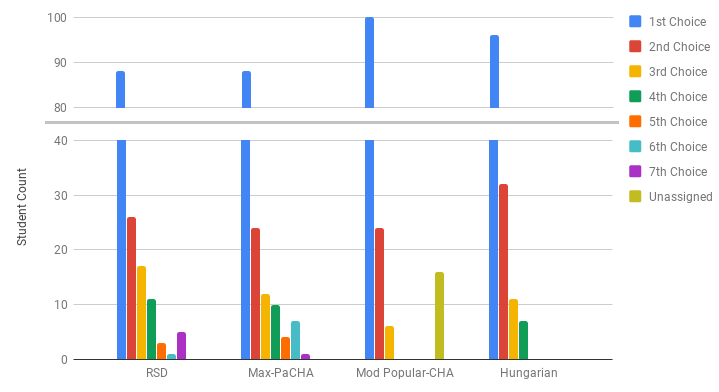
\includegraphics[width=0.75\linewidth]{assets/plots/preflib1-cropped.png}
    \caption{Rank Distribution for PrefLib1 Dataset. Note: Popular-CHA failed.}
    \label{fig:preflib1-rank-distribution}
\end{figure}

The result makes clear that Mod-Popular-CHA assigns more students to their first choice at the cost of leaving a lot of students unassigned. What else is surprising with this instance, is that the greedy RSD algorithm performs better than Max-PaCHA in regards to the rank metrics, even though both their matchings are of maximum cardinality. Surprisingly, the algorithms also tie for popularity for this instance, even though RSD performs better from a rank perspective. Runtime wise, there are no surprises other than the fact that the Hungarian algorithm is faster than Max-PaCHA for this instance. However, with this size of input, the runtime results are not that significant.

\begin{table}[h!]
  \centering
  \resizebox{\textwidth}{!}{%
  \begin{tabular}{|l|l|l|l|l|l|}
  \hline
  Metric & RSD & Max-PaCHA & Hungarian & Popular-CHA & Mod-Popular-CHA \\ \hline
  Average Rank & 1.787 & 1.924 & \cellcolor[HTML]{9AFF99}1.513 & \cellcolor[HTML]{FFCCC9}n/a & 1.276 (2.342) \\ \hline
  Rank SD & 1.136 & 1.426 & \cellcolor[HTML]{9AFF99}0.829 & \cellcolor[HTML]{FFCCC9}n/a & 0.540 (3.079) \\ \hline
  Unassigned-Count & 0 & 0 & 0 & \cellcolor[HTML]{FFCCC9}146 & \cellcolor[HTML]{FFCCC9}16 \\ \hline
  Runtime & <1ms & 19ms & 13ms & 1ms & 1ms \\ \hline
  More Popular & 1.5 & 1.5 & \cellcolor[HTML]{9AFF99}3.5 & 0 & \cellcolor[HTML]{9AFF99}3.5 \\ \hline
  Worst Rank & 7 & 7 & 4 & - & 3 / Unassigned \\ \hline
  Exists & yes & yes & yes & \cellcolor[HTML]{FFCCC9}no & yes \\ \hline
  \end{tabular}%
  }
  \caption{Summary of the Results for PrefLib1}
  \label{tab:results-preflib1}
\end{table}

Table \ref{tab:results-preflib1} shows the results in detail. Unfortunately, the Popular-CHA algorithm does not find a matching, but we can also see that the Mod-Popular-CHA algorithm finds a matching that ties in popularity with the matching produced by the Hungarian algorithm. Unsurprisingly, in terms of rank, the Hungarian algorithm produces the best matching with an average rank of 1.513 and a standard deviation of 0.829. When not taking the unassigned students into account, Mod-Popular-CHA performs even better on the rank metrics; however, when taking the unassigned students into account, it performs worst among all algorithms.


\paragraph{PrefLib2 Dataset}
Figure \ref{fig:preflib2-rank-distribution} shows the preference distribution of all five algorithms using the PrefLib2 dataset. We can see that RSD and Max-PaCHA assign some students to their 4th or 5th choice, which explains why they perform worse in terms of rank. Unsurprisingly, the matching produced by the Hungarian algorithm has the best rank-profile; however, the differences in profile among the algorithms are not that significant compared to the PrefLib1 dataset.

\begin{figure}[h!]
  \centering
    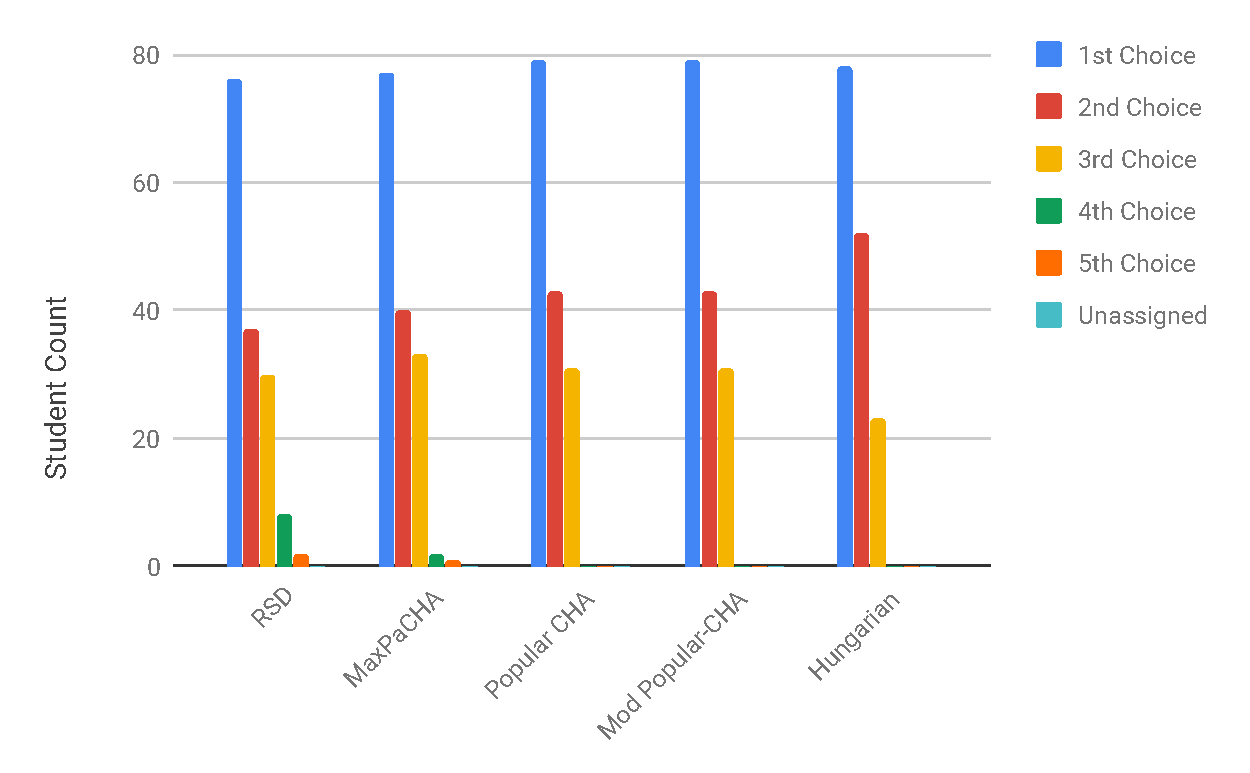
\includegraphics[width=0.9\linewidth]{assets/plots/preflib2-ranks.pdf}
    \caption{Rank Distribution for PrefLib2 Dataset.}
    \label{fig:preflib2-rank-distribution}
\end{figure}

Table \ref{tab:results-preflib2} shows the results for the PrefLib2 dataset in more detail. We can see that the Popular-CHA algorithm finds a matching, which is why the last two columns are identical. What's interesting about the results is that the matchings produced by the Hungarian and Popular-CHA algorithm tie in popularity, even though they are different in regards to the rank metrics. 

\begin{table}[h!]
  \centering
  \resizebox{\textwidth}{!}{%
  \begin{tabular}{|l|l|l|l|l|l|}
  \hline
  Metric & RSD & Max-PaCHA & Hungarian & Popular-CHA & Mod-Popular-CHA \\ \hline
  Average Rank & 1.712 & \cellcolor[HTML]{FFCCC9}1.758 & \cellcolor[HTML]{9AFF99}1.640 & 1.686 & 1.686 \\ \hline
  Rank SD & 0.797 & \cellcolor[HTML]{FFCCC9}0.878 & \cellcolor[HTML]{9AFF99}0.728 & 0.787 & 0.787 \\ \hline
  Unassigned-Count & 0 & 0 & 0 & 0 & 0 \\ \hline
  Runtime & <1ms & 41ms & 45ms & 9ms & 10ms \\ \hline
  More Popular & 1 & 0 & \cellcolor[HTML]{96FFFB}2 (+2 Ties) & \cellcolor[HTML]{96FFFB}2 (+2 Ties) & \cellcolor[HTML]{96FFFB}2 (+2 Ties) \\ \hline
  Worst Rank & 5 & 5 & 3 & 3 & 3 \\ \hline
  Exists & yes & yes & yes & yes & yes \\ \hline
  \end{tabular}%
  }
  \caption{Summary of the Results for PrefLib2}
  \label{tab:results-preflib2}
\end{table}

What also stands out is that RSD again produces a better matching than Max-PaCHA in regards to the rank metrics. In fact, the matching produced by Max-PaCHA performs worst in terms of rank, even though its runtime is the second highest. Overall, the runtimes are still low, with all of them being lower than 50ms, which should make all algorithms suitable for real world applications for similarly sized instances. However, it should be noted that the matching produced by RSD gets close in terms of rank to the matching produced by the Hungarian algorithm, even though it is nearly 50 times faster.

\subsubsection{Zipfian Datasets}
Since the Zipfian datasets have a somewhat similar preference distribution as the PrefLib datasets, we should see similar results; however, parameters can be tuned, such as preference list length and student count.

\paragraph{Small Zipfian Datasets}
We begin by looking at a similarly sized dataset as the PrefLib datasets, and then begin deviating the student \& seminar count. Figure \ref{fig:zipfian-small-distribution} shows the average ranks for 50 test runs using the Zipfian dataset with 10 seminars and about 200 students. 

\begin{figure}[h!]
  \centering
    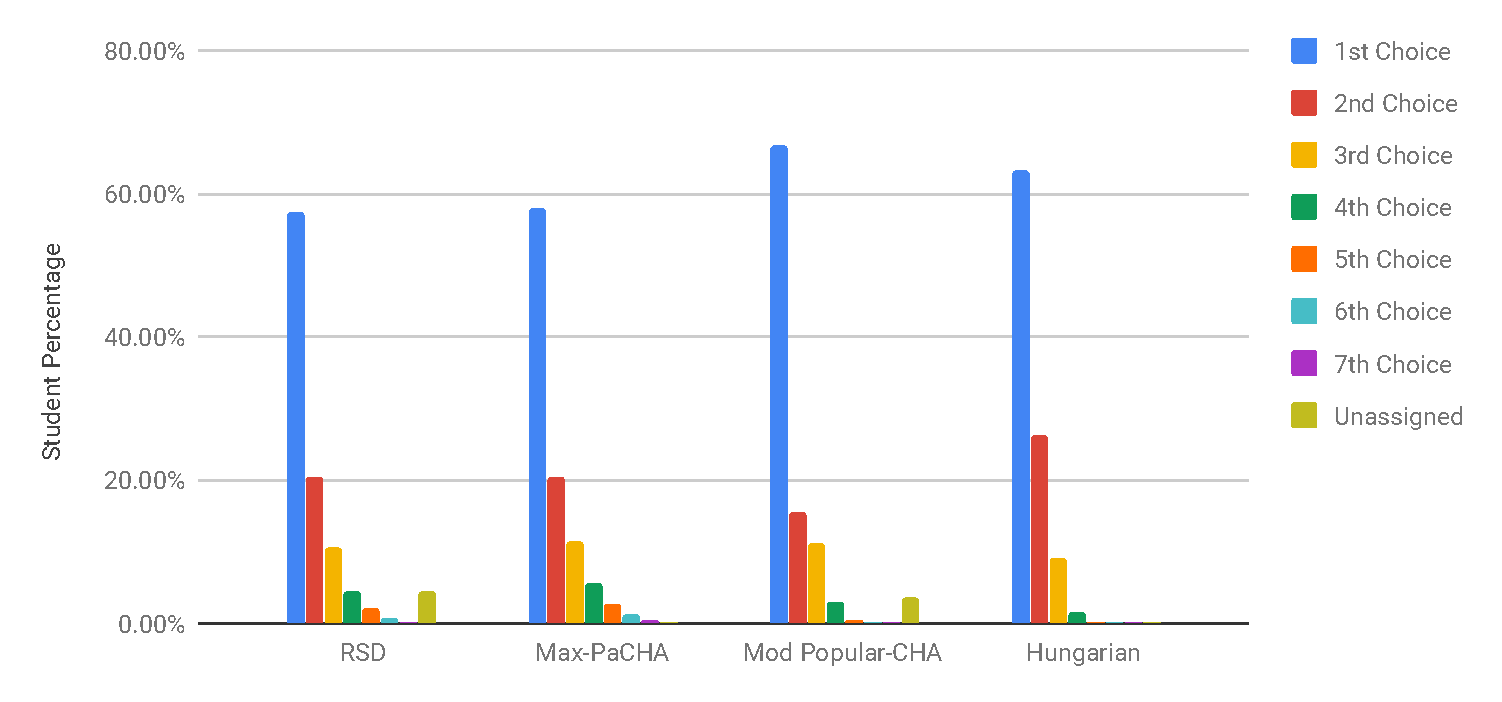
\includegraphics[width=0.8\linewidth]{assets/plots/small-zipfian-cropped.pdf}
    \caption{Rank Distribution for the Small Zipfian Dataset.}
    \label{fig:zipfian-small-distribution}
\end{figure}

We can clearly see that the Hungarian algorithm performs best in terms of worst-rank and profile in general; however, Mod-Popular-CHA assigns more students to their first choice at the cost of leaving on average 7 students unassigned.

\begin{table}[h!]
  \centering
  \resizebox{\textwidth}{!}{%
  \begin{tabular}{|l|l|l|l|l|l|}
  \hline
  Metric & RSD & Max-PaCHA & Hungarian & Popular-CHA & Mod-Popular-CHA \\ \hline
  Average Rank & 1.893 (2.014) & 1.910 & \cellcolor[HTML]{9AFF99}1.481 & 1.646 & 1.523 (1.913) \\ \hline
  Rank SD & 1.451 (1.782) & 1.457 & \cellcolor[HTML]{9AFF99}0.716 & 1.034 & 0.874 (2.121) \\ \hline
  Unassigned-Count & 2 & 0 & 0 & 0 & \cellcolor[HTML]{FFCCC9}7 \\ \hline
  Runtime & \textless{}1ms & 54ms & 60ms & 7ms & 10ms \\ \hline
  More Popular & 1 & 1.65 & 3.05 & 0.7 & \cellcolor[HTML]{9AFF99}3.6 \\ \hline
  Worst Rank & \cellcolor[HTML]{FFCCC9}8 & \cellcolor[HTML]{FFCCC9}8 & \cellcolor[HTML]{9AFF99}5 & \cellcolor[HTML]{9AFF99}5 & 6 \\ \hline
  Exists & yes & yes & yes & \cellcolor[HTML]{FFCCC9}4/50 exist & yes \\ \hline
  \end{tabular}%
  }
  \caption{Average Results for the Small Zipfian Dataset with 50 Runs}
  \label{tab:results-zipfian-small}
\end{table}

Table \ref{tab:results-zipfian-small} shows the average results in more detail and shows that, out of the 50 instances, Popular-CHA only finds a matching for four instances. When it finds a matching, it does so quite fast, and the matching is, on average, better rank-wise than all matchings produced by the other algorithms, except for the ones produced by the Hungarian algorithm. In terms of popularity, Mod-Popular-CHA actually outperforms all algorithms (equal to Popular-CHA if the matching exists) for most instances, even though rank-wise it does not perform as well as the Hungarian algorithm. However, the Hungarian algorithm produces more popular matchings than most other algorithms, and, for some instances, even more popular ones than the Mod-Popular-CHA algorithm.

\paragraph{Large Zipfian Datasets}
Using a large dataset with a Zipfian distribution yields similar results. Figure \ref{fig:zipfian-medium-distribution} shows the rank distributions for 10 test runs with datasets that contain about 2500 students and 35 seminars. We can see that Mod Popular-CHA is able to outperform the other algorithms in terms of popularity by maximizing the number of students being assigned to their first choice. However, the Hungarian algorithm produces more balanced matchings, where most students are assigned to their top three choices, while also leaving no student unassigned.

\begin{figure}[h!]
  \centering
    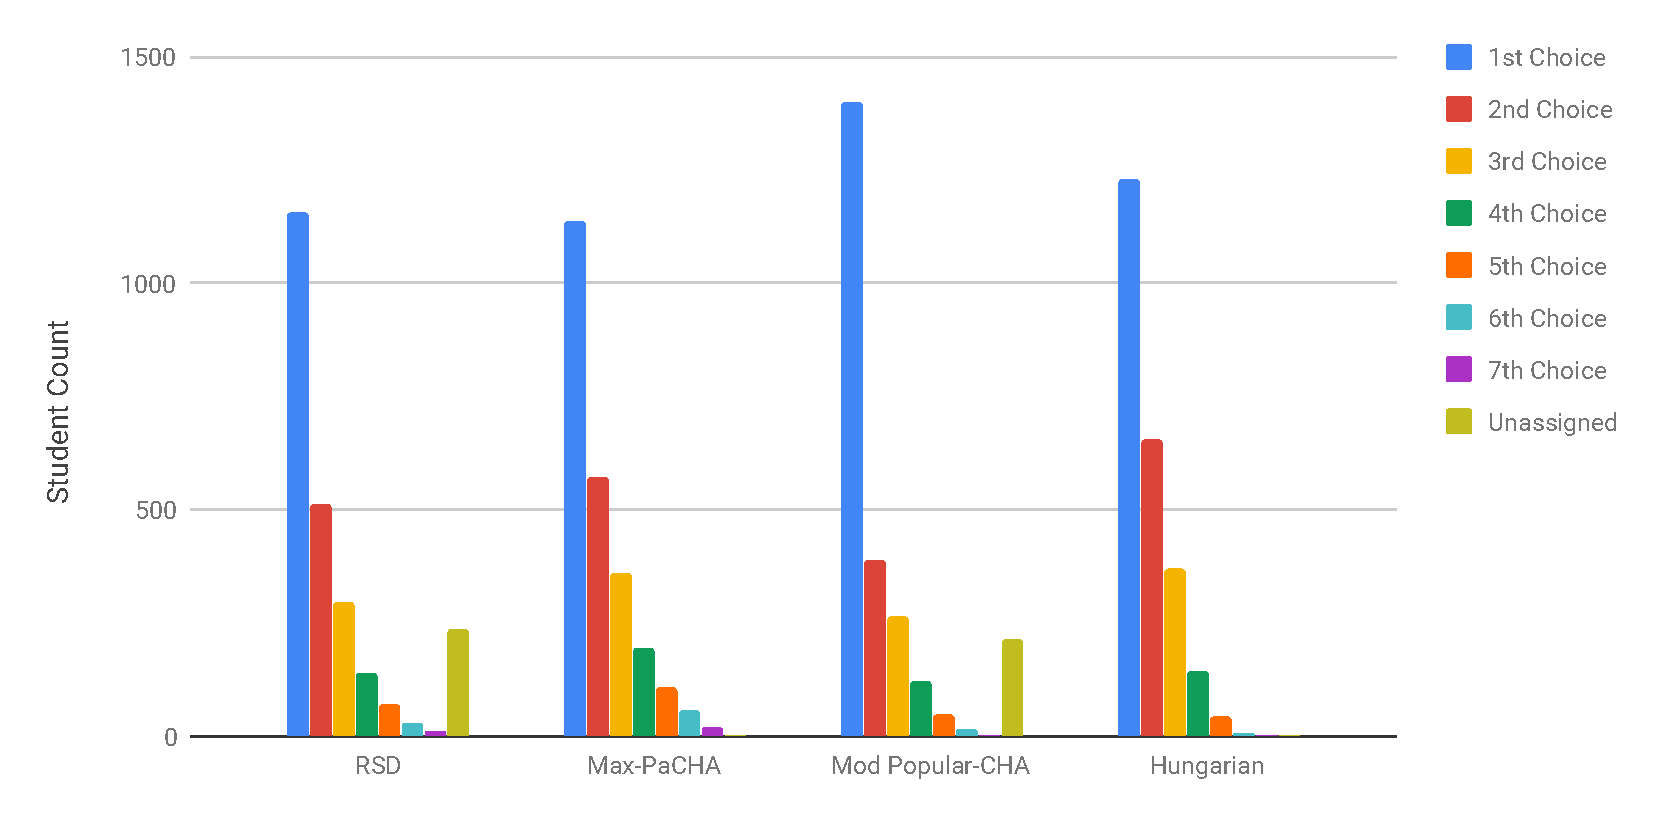
\includegraphics[width=0.8\linewidth]{assets/plots/zipfian-medium.pdf}
    \caption{Rank Distribution for the Large Zipfian Datasets.}
    \label{fig:zipfian-medium-distribution}
\end{figure}

\begin{table}[h!]
  \centering
  \resizebox{\textwidth}{!}{%
  \begin{tabular}{|l|l|l|l|l|l|}
  \hline
  Metric & RSD & Max-PaCHA & Hungarian & Popular-CHA & Mod-Popular-CHA \\ \hline
  Average Rank & 1.911 (5.287) & \cellcolor[HTML]{FFCCC9}2.109 & \cellcolor[HTML]{9AFF99}1.824 & - & 1.694 (4.746) \\ \hline
  Rank SD & 1.225 (10.41) & \cellcolor[HTML]{FFCCC9}1.383 & \cellcolor[HTML]{9AFF99}1.029 & - & 1.087 (9.967) \\ \hline
  Unassigned & \cellcolor[HTML]{FFCCC9}10\% & \cellcolor[HTML]{9AFF99}0\% & \cellcolor[HTML]{9AFF99}0\% & 100\% & \cellcolor[HTML]{FFCCC9}8.6\% \\ \hline
  Runtime & \cellcolor[HTML]{9AFF99}3ms & 2190ms & \cellcolor[HTML]{FFCCC9}65730ms & - & \cellcolor[HTML]{9AFF99}168ms \\ \hline
  More Popular & 1.1 & 1.65 & 3 & 0 & \cellcolor[HTML]{9AFF99}4 \\ \hline
  Worst Rank & 7 & 7 & \cellcolor[HTML]{9AFF99}6 & - & 7 \\ \hline
  Exists & yes & yes & yes & \cellcolor[HTML]{FFCCC9}0/10 & yes \\ \hline
  \end{tabular}%
  }
  \caption{Average Results for the Large Zipfian Dataset (2500 Students) with 10 Runs}
  \label{tab:results-zipfian-medium}
\end{table}

Table \ref{tab:results-zipfian-medium} summarizes the results in detail and shows that Popular-CHA is not very successful and finds no matching in any of the test runs. However, Mod-Popular-CHA always produces more popular matchings than all of the other algorithms, even though 8.6\% of the students were left unassigned on average. When taking the unassigned students out of the rank metrics, Mod-Popular-CHA produces matchings with the best average rank and standard deviation, while having the second lowest runtime. In contrast to that, the Hungarian algorithm always assigns all students, even though it takes, on average, 65 seconds to do so. This confirms the theoretical observations about runtime and shows that using the Hungarian algorithm is potentially less desirable for large instances.

\subsubsection{Large Uniform Datasets}

\paragraph{Datasets with Incomplete Preferences}
This large uniform dataset contains 50 seminars and 5000 students, who each randomly pick 10 seminars with equal probability.

\begin{figure}[h!]
  \centering
    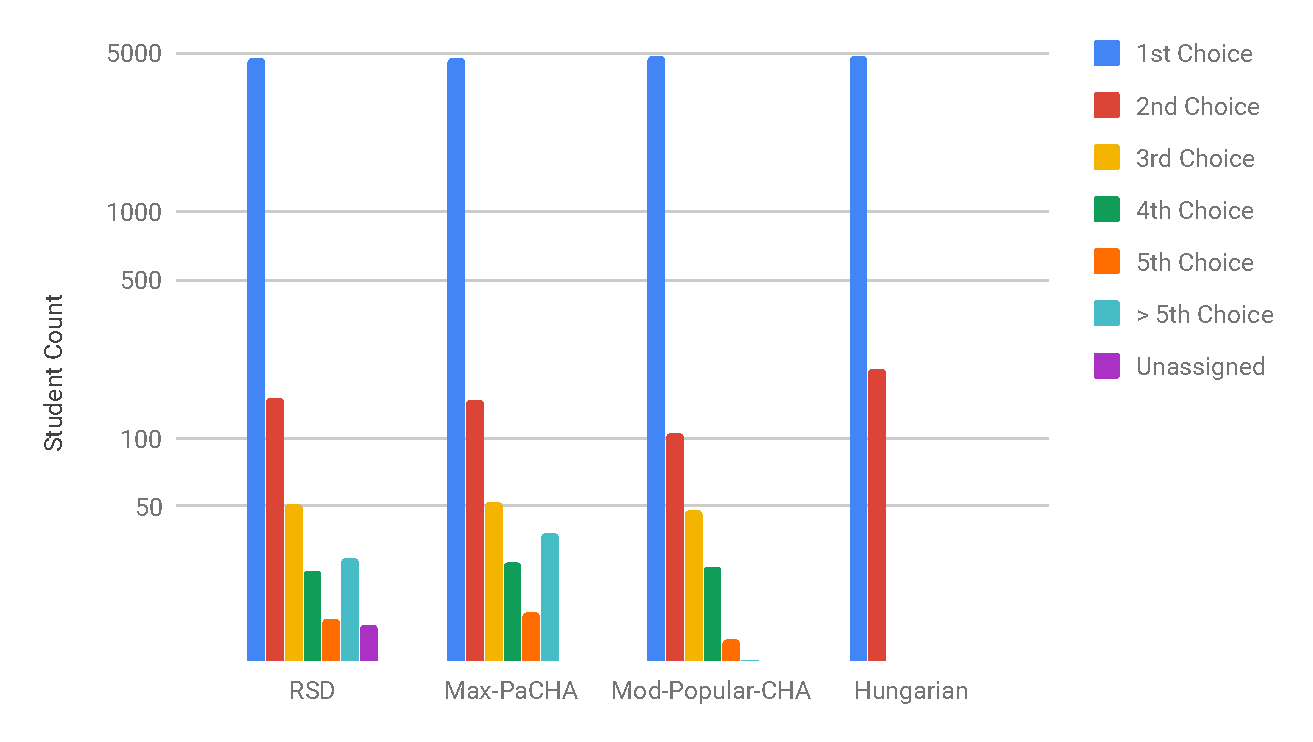
\includegraphics[width=0.75\linewidth]{assets/plots/uniform_incompl_distr.pdf}
    \caption{Rank Distribution on Log-Scale for the Uniform Dataset with Incomplete Preferences.}
    \label{fig:uniform-incomplete-distribution}
\end{figure}

Figure \ref{fig:uniform-incomplete-distribution} shows the average ranks when executing each algorithm 10 times using incomplete preference lists. We can see that all algorithms assign a vast majority (94\%) of students to their first choice; however, all algorithms, but the Hungarian algorithm, also assign students to their lower preferences and therefore have a worse profile.

\begin{table}[h!]
  \centering
  \resizebox{\textwidth}{!}{%
  \begin{tabular}{|l|l|l|l|l|l|}
  \hline
  Metric & RSD & Max-PaCHA & Hungarian & Popular-CHA & Mod-Popular-CHA \\ \hline
  Average Rank & 1.119 (1.265) & \cellcolor[HTML]{FFCCC9}1.133 & \cellcolor[HTML]{9AFF99}1.041 & 1.093 & 1.083 \\ \hline
  Rank SD & 0.647 (2.778) & \cellcolor[HTML]{FFCCC9}0.713 & \cellcolor[HTML]{9AFF99}0.2 & 0.508 & 0.486 \\ \hline
  Unassigned & 0.28\% & 0\% & 0\% & 0\% (90\%) & 0\% \\ \hline
  Runtime & 13ms & 6175ms & \cellcolor[HTML]{FFCCC9}55815ms & 257ms & 221ms \\ \hline
  More Popular & 1.65 & 1.15 & \cellcolor[HTML]{9AFF99}3.45 & 0.3 & \cellcolor[HTML]{9AFF99}3.45 \\ \hline
  Worst Rank & 10 & 10 & \cellcolor[HTML]{9AFF99}2 & 8 & 10 \\ \hline
  Exists & yes & yes & yes & 1/10 & yes \\ \hline
  \end{tabular}%
  }
  \caption{Average Results for the Large Uniform Datasets with Incomplete Preferences.}
  \label{tab:results-uniform-large}
\end{table}

In Table \ref{tab:results-uniform-large} we can see that Popular-CHA only finds a matching for one out of the 10 instances, but when it does, it performs quite well in terms of rank. However, Mod-Popular-CHA is on average able to find better matchings in less time than Popular-CHA. What also stands out is that Mod-Popular-CHA and the Hungarian algorithm are tied for popularity for every instance, but runtime-wise, Mod-Popular-CHA performs far better than the Hungarian algorithm.

\paragraph{Datasets with Complete Preferences}
When using the same size dataset as before, but with complete preference lists, the results show some interesting insights.

\begin{figure}[h!]
  \centering
    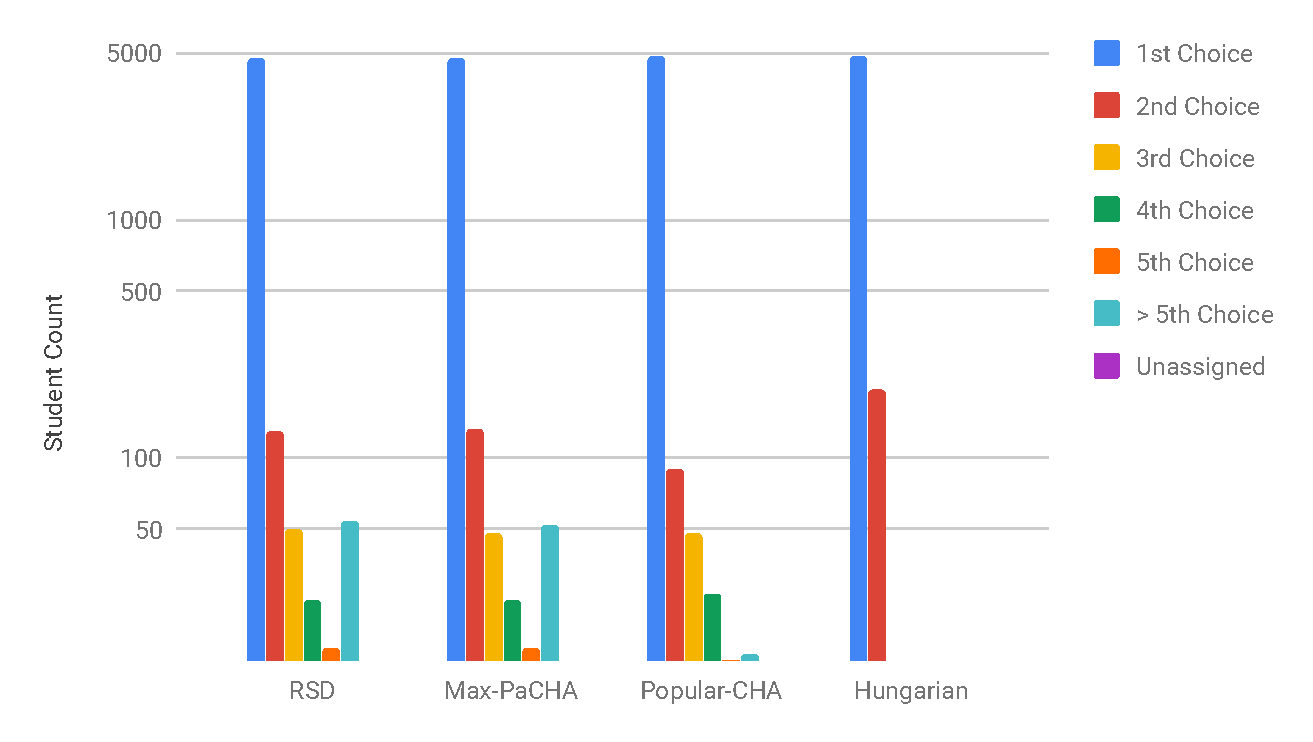
\includegraphics[width=0.75\linewidth]{assets/plots/uniform_compl_distr.pdf}
    \caption{Rank Distribution on Log-Scale for the Uniform Dataset with Complete Preferences.}
    \label{fig:uniform-complete-distribution}
\end{figure}

Figure \ref{fig:uniform-complete-distribution} shows the average ranks when executing each algorithm 10 times using complete preference lists. We see the same pattern as with incomplete preferences, namely that the Hungarian algorithm's matchings have the best profile and a low worst rank of two. Compared to that RSD and Max-PaCHA assign around 50 students to their 5th choice or worse.

Besides that, Table \ref{tab:results-uniform-large-complete} shows that Popular-CHA finds a matching for every instance, which helps answer the question if preference list length has an effect on Popular-CHA. For this dataset, Popular-CHA and the Hungarian algorithm always produce matchings of the same popularity, which means that there exists more than one popular matching for every instance. 

\begin{table}[h!]
  \centering
  \resizebox{\textwidth}{!}{%
  \begin{tabular}{|l|l|l|l|l|l|}
  \hline
  Metric & RSD & Max-PaCHA & Hungarian & Popular-CHA & Mod-Popular-CHA \\ \hline
  Average Rank & \cellcolor[HTML]{FFCCC9}1.198 & 1.190 & \cellcolor[HTML]{9AFF99}1.039 & \cellcolor[HTML]{9AFF99}1.076 & \cellcolor[HTML]{9AFF99}1.076 \\ \hline
  Rank SD & \cellcolor[HTML]{FFCCC9}1.543 & 1.469 & \cellcolor[HTML]{9AFF99}0.193 & \cellcolor[HTML]{9AFF99}0.453 & \cellcolor[HTML]{9AFF99}0.453 \\ \hline
  Unassigned & 0\% & 0\% & 0\% & 0\% & 0\% \\ \hline
  Runtime & 11ms & 7922ms & \cellcolor[HTML]{FFCCC9}57141ms & 228ms & 219ms \\ \hline
  More Popular & 0.5 & 0.5 & \cellcolor[HTML]{9AFF99}3 & \cellcolor[HTML]{9AFF99}3 & \cellcolor[HTML]{9AFF99}3 \\ \hline
  Worst Rank & \cellcolor[HTML]{FFCCC9}30 & \cellcolor[HTML]{FFCCC9}27 & \cellcolor[HTML]{9AFF99}2 & 9 & 9 \\ \hline
  Exists & yes & yes & yes & \cellcolor[HTML]{9AFF99}10/10 & yes \\ \hline
  \end{tabular}%
  }
  \caption{Average Results for Large Uniform Dataset with Complete Preferences.}
  \label{tab:results-uniform-large-complete}
\end{table}

Another thing that stands out is the fact that RSD and Max-PaCHA find matchings with high worst-ranks of 30 and 27 respectively. Overall, these two algorithms perform worse than or equal to the Popular-CHA and Hungarian algorithm on all metrics, which makes them less appealing for this kind of dataset. Given the low average runtime of 219ms, Mod-Popular-CHA seems to be a good option when the size of the instance is too large for the Hungarian algorithm, while still performing well on the rank-related metrics. Even though Popular-CHA and the Hungarian algorithm tie in popularity, it should be assumed that a matching with the worst rank of 2 is more preferred among the students than a matching with a worst rank of 9. 

\subsection{Conclusions of Experiments}
In summary, the matchings produced by the Hungarian algorithm usually perform best in all of the metrics, except for runtime, where it performs the worst by far. However, for the student seminar use case, that should not be a problem, because most instances will be smaller than the large datasets that we have tested with. In fact, when using the real-world datasets (see Table \ref{tab:results-preflib1} and \ref{tab:results-preflib2}), the runtime differences for the different mechanisms are insignificant. For large instances, the modified Popular-CHA algorithm performs well and could be optimized even further for matching more students. The Mod-Popular-CHA algorithm, as it was described in Section \ref{impl:mod-max-pop}, does not try to assign students that were left unmatched when finding a maximum-cardinality matching. This could easily be improved by either using a simple mechanism like RSD, or even using the Hungarian algorithm on the set of unassigned students to increase the cardinality of the matching. Neither modification guarantees that the final matching would be popular or of maximum cardinality, but it could improve the result. Therefore, it would make the Mod-Popular-CHA algorithm a fast heuristic that should, according to the experiments, perform better than RSD and Max-PaCHA for most instances, while still keeping the runtime low.

\begin{figure}[h!]
  \centering
    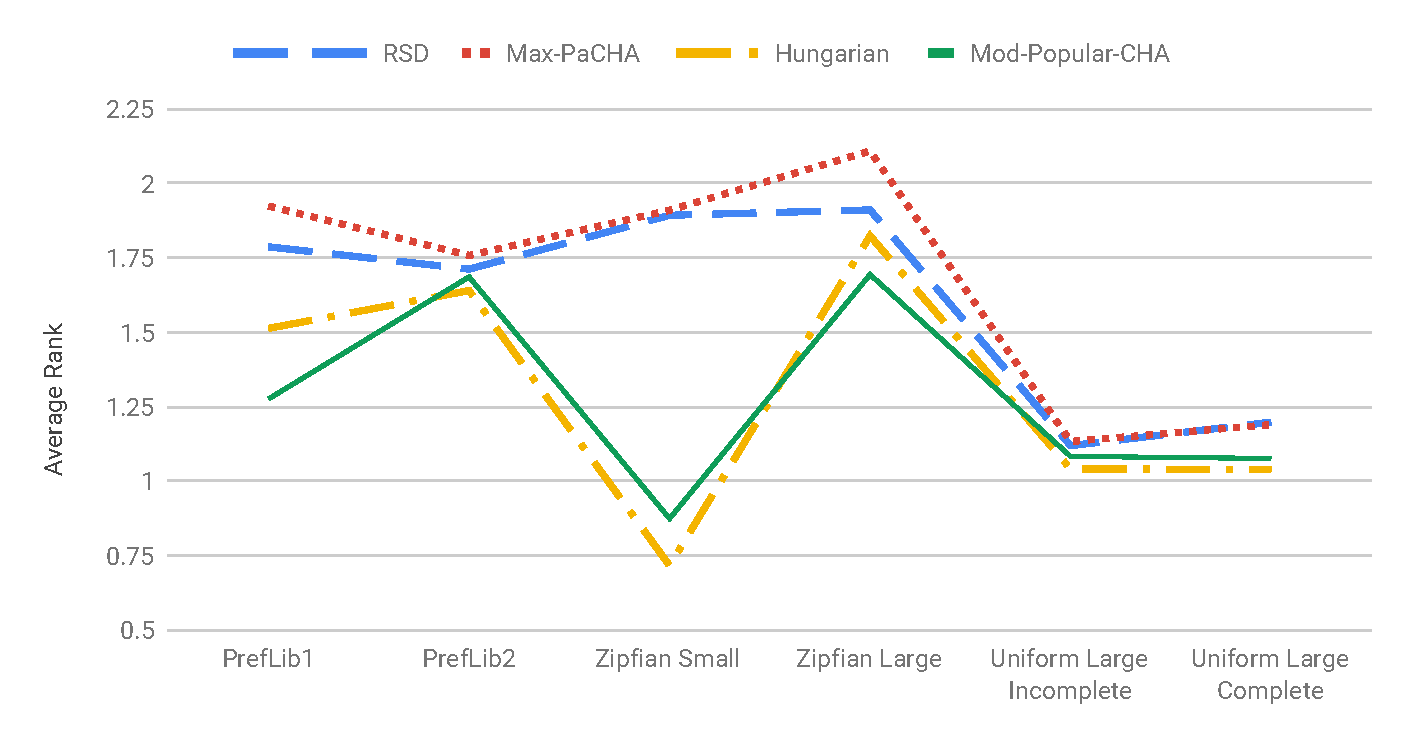
\includegraphics[width=0.8\linewidth]{assets/plots/average_ranks_all.pdf}
    \caption{Average Rank Comparison between Algorithms and Datasets.}
    \label{fig:average_ranks}
\end{figure}

In terms of average rank, Figure \ref{fig:average_ranks} summarizes the average ranks for each dataset and algorithm, except for Popular-CHA. We can see that for some instances, the differences in rank are not very significant, but for other instances the difference is noteworthy. Unsurprisingly, the Hungarian algorithm generally performs the best; however, for two types of datasets, Mod-Popular-CHA beats the Hungarian algorithm in the average rank metric at the cost of leaving students unassigned. Still, the Hungarian algorithm produces matchings with the lowest rank standard deviation, i.e. lowest fluctuation of rank, which makes this mechanism the fairest towards all students.

\subsubsection{Answers to the Research Questions}
The experiments reveal some interesting insights that should help answering the research questions from Section \ref{sec:research-q}.

\paragraph{Effect of Different Preference Distributions:} Unsurprisingly, the algorithms perform better on the rank metrics when the preferences are distributed uniformly - in fact, the Hungarian algorithm is able to assign on average more than 94\% (Table \ref{tab:results-uniform-large-complete}) of the students to their first choice when the preference distribution was uniform.
\paragraph{Failure Rate of Popular-CHA:} The experiments show that \mbox{Popular-CHA} fails to find a matching quite often, especially if the preference lists are short and not uniformly distributed. When using the Zipfian datasets (Tables \ref{tab:results-zipfian-medium}, \ref{tab:results-zipfian-small}), Popular-CHA only finds a matching for 4/50 instances. Even for uniform distributions and incomplete preference lists (Table \ref{tab:results-uniform-large}), the algorithm only finds a matching for 1/10 instances. Making the preference lists complete makes it easier for the algorithm to find matchings as shown in Table \ref{tab:results-uniform-large-complete}.
\paragraph{Performance of Mod-Popular-CHA:} The modified version of Popular-CHA was able to find comparatively good matchings in a short amount of time, while typically also producing more or equally popular matchings as the other algorithms. For many instances, Mod-Popular-CHA ties the Hungarian algorithm for popularity and was able to produce good matchings in terms of the rank metrics in a fraction of the time.
\paragraph{Cost of Giving up on Strategy-proofness:} Surprisingly, RSD produces, on average, better matchings on most metrics than Max-PaCHA, while also being by far the fastest algorithm. However, RSD usually produces the highest percentage of unassigned students; additionally, the modified Popular-CHA algorithm typically outperforms RSD on most metrics, while also having a relatively low runtime. In the real-world datasets (PrefLib), RSD leaves no students unassigned and gets close to the Hungarian algorithm in terms of rank, but also produced 7 as the worst rank, compared to 4 for the Hungarian algorithm. 
\paragraph{Popularity as a Meaningful Metric:} For many instances, we cannot find the one popular matching, as Popular-CHA simply fails - but when it does find a matching, the worst rank, average rank and rank standard deviation is higher than what the Hungarian algorithm produces. Another interesting insight is that matchings produced by Mod-Popular-CHA usually tie in popularity with those produced by the Hungarian algorithm, even though Mod-Popular-CHA often left a few students unassigned. For instance, in Figure \ref{fig:zipfian-medium-distribution}, Mod-Popular-CHA leaves, on average, 8.6\% of the students unassigned, but the matchings are still classified as more popular than, or, just as popular as the matchings produced by the Hungarian algorithm. This shows that a popular matching can maximize the number of students ranked to their first choice at the cost of some students being matched to a low-ranking seminar, or even no seminar at all. This makes it questionable as to whether or not popularity is a meaningful optimality criterion for the student and seminar use case, as it should be a goal to assign as many students as possible and to make all students equally satisfied with their match, instead of finding the biggest possible subset of satisfied students.
\paragraph{The Effect of Short Preference Lists:} The experiments show that short preference lists make it more likely for Popular-CHA to not find a matching, as well as making it more likely for RSD to produce matchings with more unassigned students.
